% Drawing 154/06-26 -- folder 154, batch 06, archive page 110 (PDF page 111).
% Transcription: à droite, sous « $n - 1$ », un rectangle vert clair dont les grands côtés, renforcés en brun et coupés de petits traits rouges, sont marqués $n - \nu$, et les petits côtés, en gros pointillé noir, $(\nu - 1)$ ; à droite « $(\nu - 1) + 1$ »
% Kind: rectangle with sides n - nu and nu - 1. Method 2 (schematic redraw from the facsimile). Status: ok.
% Notes: Light green rectangle, a black point at each corner; the long sides doubled by a brown stroke and cut by small red ticks (four on the upper side), the short sides doubled by a thick black dotted stroke; n - nu above and below, (nu - 1) at the left, (nu - 1) + 1 at the right; n - 1 above left. The second « n - 1 », struck out on the page, is not drawn. Redrawn 2026-11-12 (issue 128): to check again.
% Coordinates: 1 unit = 1 mm = 1/100 of the crop width (bbox in page fractions: [0.555, 0.125, 0.8, 0.215]).
% Redrawn by Claude (claude-fable-5-2), issue #128, 2026-11-12; not checked by a human; not compiled (no TeX in the session).
% Rights: reproduces part of the work -- behind RENDER_TRANSCRIPTS, never published by itself.
\documentclass[tikz,border=3pt]{standalone}
\usepackage{amsmath,amssymb}
\usetikzlibrary{patterns,arrows.meta}
\tikzset{Lg/.style={green!60!black!70}, Br/.style={brown!80!black}, Rd/.style={red!85!black}, pencil/.style={black!45}, struck/.style={black!35}, mpt/.style={circle,draw,inner sep=1.3pt}, pt/.style={circle,fill,inner sep=0.9pt}, opt/.style={circle,draw,fill=white,inner sep=1.1pt}}
\begin{document}
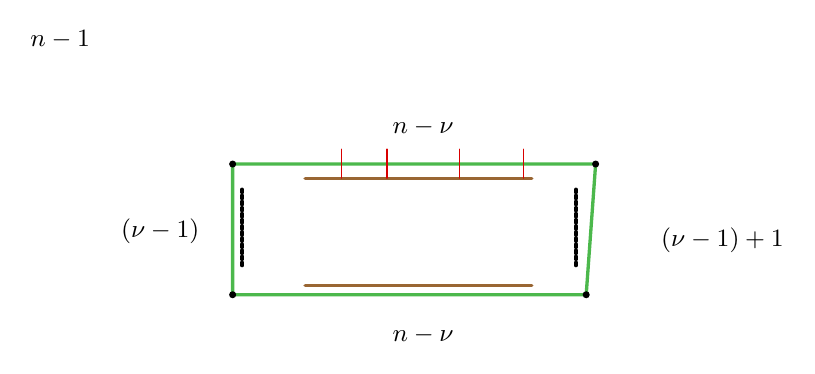
\begin{tikzpicture}[x=1mm,y=1mm,line cap=round,line join=round,font=\scriptsize]
\draw[Lg,very thick] (19.2,-21.1) -- (65.3,-21.1) -- (64.1,-37.7) -- (19.2,-37.7) -- cycle;
\draw[Br,very thick] (28.4,-22.9) -- (57.2,-22.9);
\draw[Br,very thick] (28.4,-36.5) -- (57.2,-36.5);
\draw[Rd] (33,-19.2) -- (33,-22.9);
\draw[Rd] (38.8,-19.2) -- (38.8,-22.9);
\draw[Rd] (48,-19.2) -- (48,-22.9);
\draw[Rd] (56.1,-19.2) -- (56.1,-22.9);
\draw[densely dotted,very thick] (20.4,-24.3) -- (20.4,-34.2);
\draw[densely dotted,very thick] (62.8,-24.3) -- (62.8,-34.2);
\node[pt] at (19.2,-21.1) {};
\node[pt] at (65.3,-21.1) {};
\node[pt] at (64.1,-37.7) {};
\node[pt] at (19.2,-37.7) {};
\node[inner sep=1pt] at (43.4,-16.4) {\small $n-\nu$};
\node[inner sep=1pt] at (43.4,-42.8) {\small $n-\nu$};
\node[inner sep=1pt] at (10,-29.6) {\small $(\nu-1)$};
\node[inner sep=1pt] at (81.4,-30.8) {\small $(\nu-1)+1$};
\node[inner sep=1pt] at (-2.7,-5.3) {\small $n-1$};
\end{tikzpicture}
\end{document}
